\section{10 Weeks!}

We’re at that strange moment of limbo in the proceedings for the expedition, the majority of stuff that needs to be done in advance has been, the rope is washed, the gear order has been made, the ferry tickets are booked and the special permission to camp in the national park is being sort. Yet there is a massive tasks list of things that practically require doing, and almost our entire undergraduate workforce is suffering under examinations.

\margininbox{Converting WGS84}{I thought I would investigate transforming GPS/WGS84 coordinates into the local Gauss-Krueger coordinates used by the Kataster. Alas, there still isn’t a perfect solution, but I did find an interesting new wiki:

“The difference from the original Bessel’s ellipsoid (so-called Hermannskogel datum) to the current referent system (WGS84) is non-systematic.”
\name{Jarv}}{\logbook}

Stores is a disordered mess, the chaos of the Easter tour intermingling with preparations for the summer. Still, with each piece of underground comf freshly laundered and put away, to each survey instrument gently cleaned and checked, a successful \& productive summer expedition is brought ever closer.

\name{Jarvist Frost}

\begin{pagefigure}
\checkoddpage \ifoddpage \forcerectofloat \else \forceversofloat \fi
   \centering
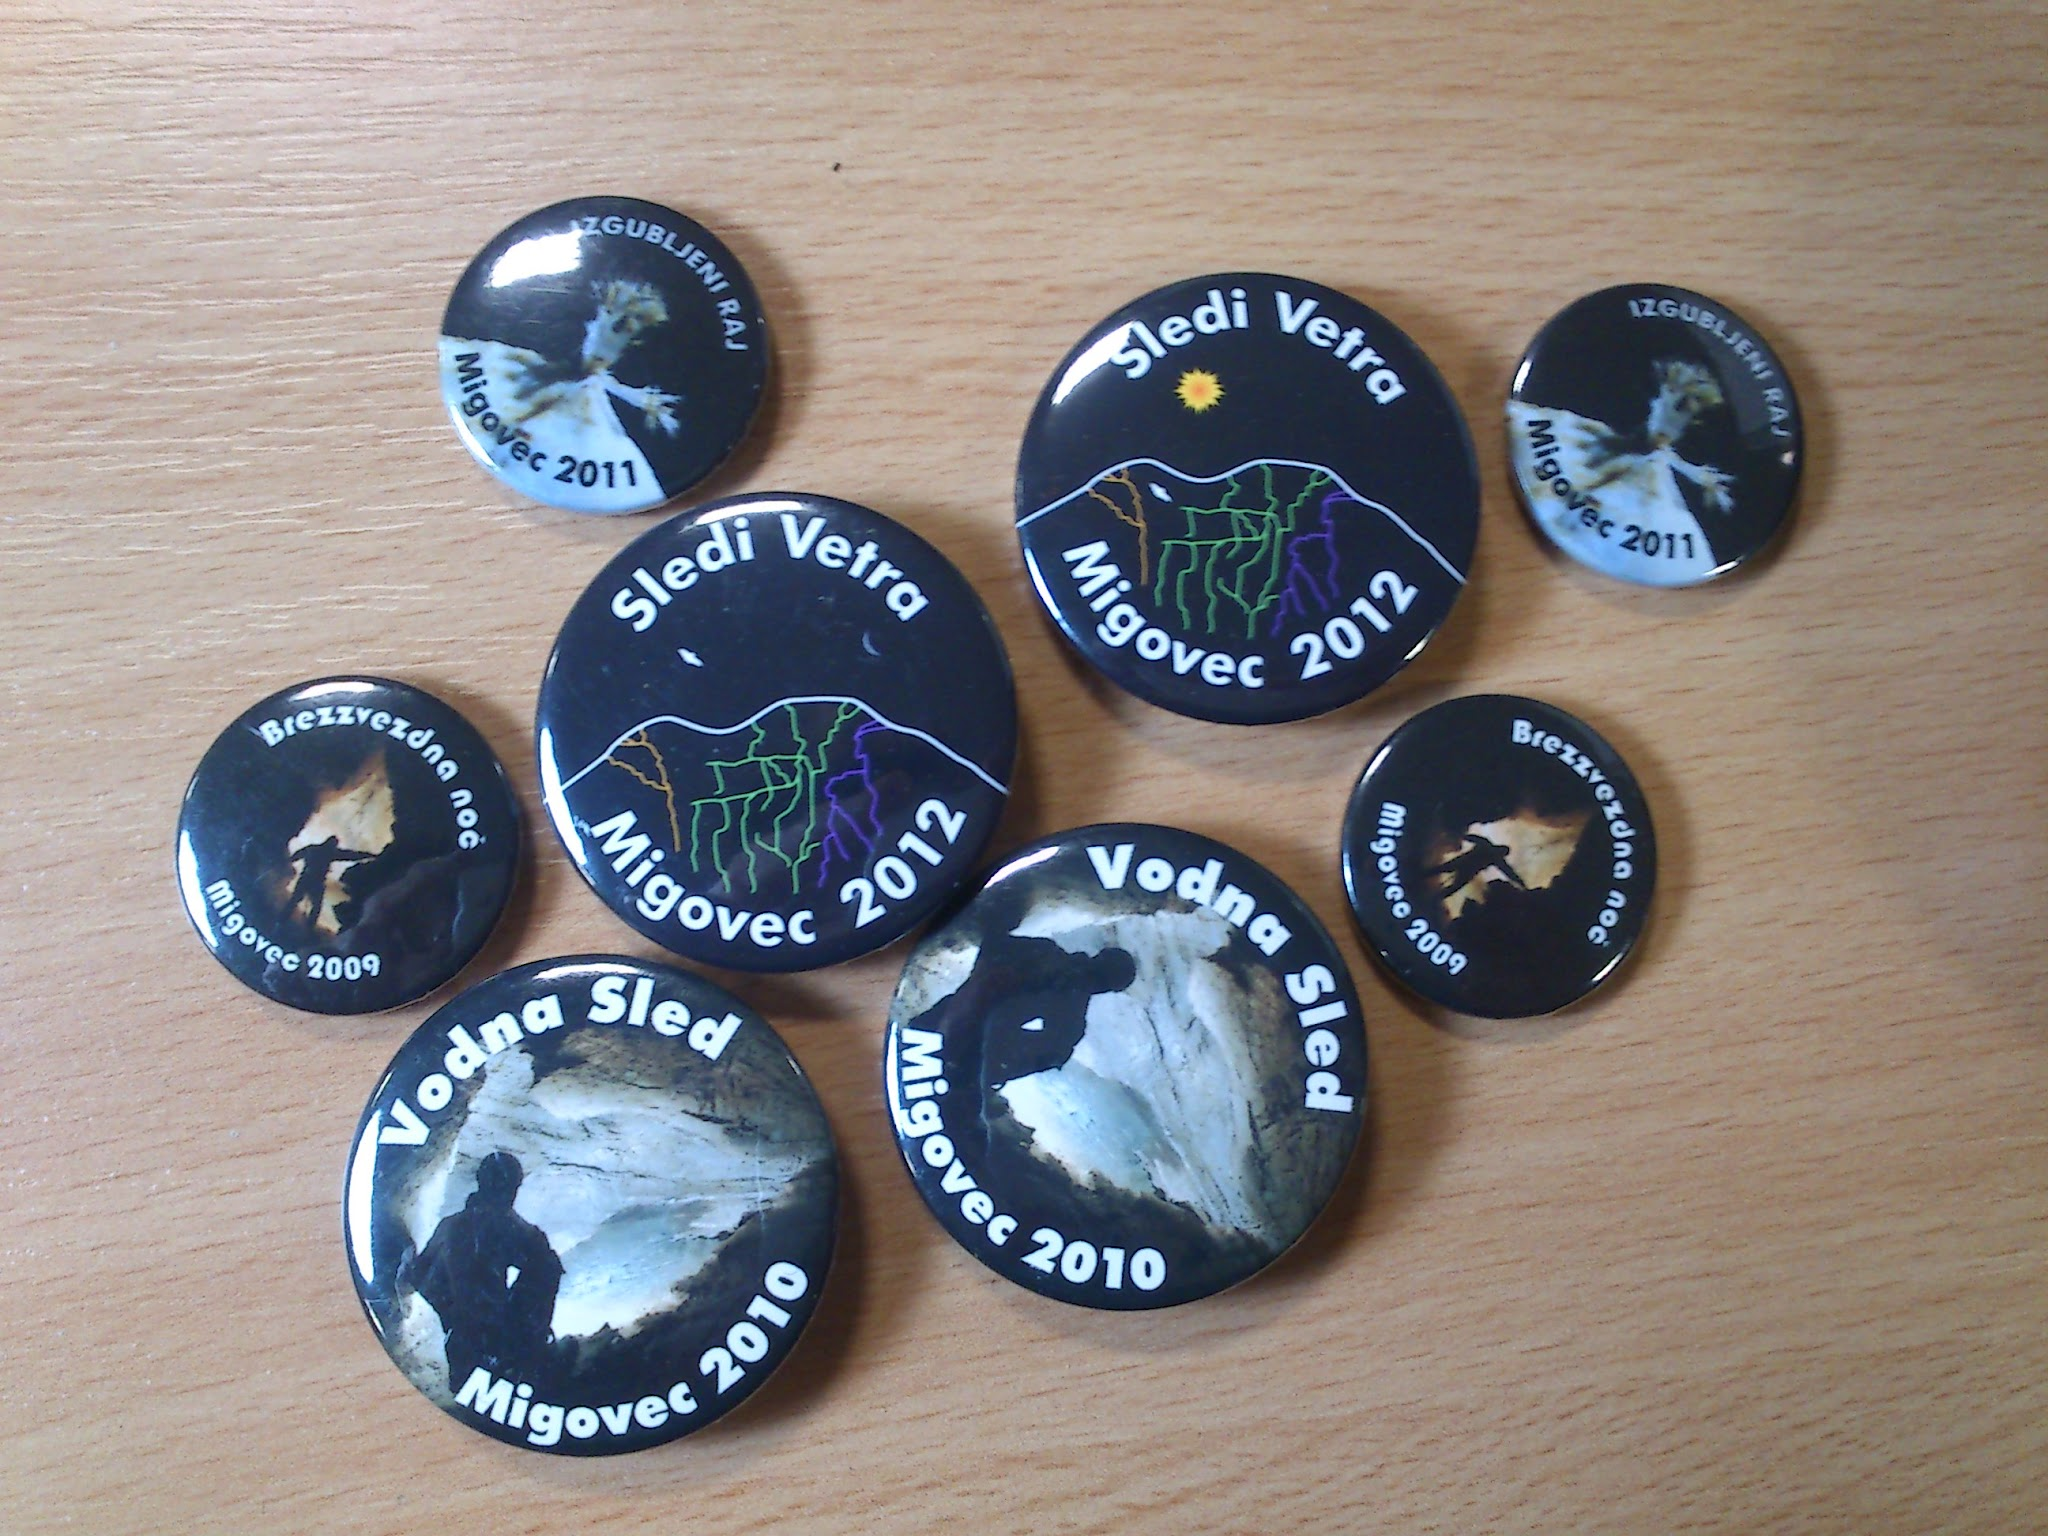
\includegraphics[width = \textwidth]{2012/10_weeks/2012-02-10-2045JarvistMooreFrost-DSC_0203--orig.jpg}
\caption{Expedition badges for 2009---2012. \pic{Jarvist Frost}} \label{expo badges}
\end{pagefigure}
